\documentclass{article}

% chinese fonts
\usepackage{ctex}

% math fonts
\usepackage{amsmath}
\usepackage{amsthm}
\usepackage{amssymb}
\usepackage{bm}

% figures
\usepackage{tikz}
\usepackage{graphicx}
\graphicspath{{./figures/}}

% tables
\usepackage{tabularx}
\usepackage{booktabs}

% codes
\usepackage{listings}

% hyperlinks
\usepackage{hyperref}
\hypersetup{
  breaklinks,
  colorlinks = true,
  citecolor  = blue,
  linkcolor  = red,
  urlcolor   = magenta,
}

% bibliography
\usepackage[sort&compress,numbers]{natbib}

% About:  Macros for Vector, Matrix, Tensor, Math Operator and Misc
% Author: Jingxuan Yang

% vectors
\newcommand{\va}{\bm{a}}       \newcommand{\vah}{\hat{\bm{a}}}        \newcommand{\ah}{\hat{a}}    \newcommand{\vat}{\tilde{\bm{a}}}       \newcommand{\at}{\tilde{a}}
\newcommand{\vb}{\bm{b}}       \newcommand{\vbh}{\hat{\bm{b}}}        \newcommand{\bh}{\hat{b}}    \newcommand{\vbt}{\tilde{\bm{b}}}       \newcommand{\bt}{\tilde{b}}
\newcommand{\vc}{\bm{c}}       \newcommand{\vch}{\hat{\bm{c}}}        \newcommand{\ch}{\hat{c}}    \newcommand{\vct}{\tilde{\bm{c}}}       \newcommand{\ct}{\tilde{c}}
\newcommand{\vd}{\bm{d}}       \newcommand{\vdh}{\hat{\bm{d}}}        \newcommand{\dhat}{\hat{d}}  \newcommand{\vdt}{\tilde{\bm{d}}}       \newcommand{\dt}{\tilde{d}}
\newcommand{\ve}{\bm{e}}       \newcommand{\veh}{\hat{\bm{e}}}        \newcommand{\eh}{\hat{e}}    \newcommand{\vet}{\tilde{\bm{e}}}       \newcommand{\et}{\tilde{e}}
\newcommand{\vf}{\bm{f}}       \newcommand{\vfh}{\hat{\bm{f}}}        \newcommand{\fh}{\hat{f}}    \newcommand{\vft}{\tilde{\bm{f}}}       \newcommand{\ft}{\tilde{f}}
\newcommand{\vg}{\bm{g}}       \newcommand{\vgh}{\hat{\bm{g}}}        \newcommand{\gh}{\hat{g}}    \newcommand{\vgt}{\tilde{\bm{g}}}       \newcommand{\gt}{\tilde{g}}
\newcommand{\vh}{\bm{h}}     \newcommand{\vhh}{\hat{\bm{h}}}        \newcommand{\hh}{\hat{h}}    \newcommand{\vht}{\tilde{\bm{h}}}       \newcommand{\htild}{\tilde{h}}
\newcommand{\vi}{\bm{i}}       \newcommand{\vih}{\hat{\bm{i}}}        \newcommand{\ih}{\hat{i}}    \newcommand{\vit}{\tilde{\bm{i}}}       \newcommand{\itild}{\tilde{i}}
\newcommand{\vj}{\bm{j}}       \newcommand{\vjh}{\hat{\bm{j}}}        \newcommand{\jh}{\hat{j}}    \newcommand{\vjt}{\tilde{\bm{j}}}       \newcommand{\jt}{\tilde{j}}
\newcommand{\vk}{\bm{k}}       \newcommand{\vkh}{\hat{\bm{k}}}        \newcommand{\kh}{\hat{k}}    \newcommand{\vkt}{\tilde{\bm{k}}}       \newcommand{\kt}{\tilde{k}}
\newcommand{\vl}{\bm{l}}       \newcommand{\vlh}{\hat{\bm{l}}}        \newcommand{\lh}{\hat{l}}    \newcommand{\vlt}{\tilde{\bm{l}}}       \newcommand{\lt}{\tilde{l}}
\newcommand{\vm}{\bm{m}}       \newcommand{\vmh}{\hat{\bm{m}}}        \newcommand{\mh}{\hat{m}}    \newcommand{\vmt}{\tilde{\bm{m}}}       \newcommand{\mt}{\tilde{m}}
\newcommand{\vn}{\bm{n}}       \newcommand{\vnh}{\hat{\bm{n}}}        \newcommand{\nh}{\hat{n}}    \newcommand{\vnt}{\tilde{\bm{n}}}       \newcommand{\nt}{\tilde{n}}
\newcommand{\vo}{\bm{o}}       \newcommand{\voh}{\hat{\bm{o}}}        \newcommand{\oh}{\hat{o}}    \newcommand{\vot}{\tilde{\bm{o}}}       \newcommand{\ot}{\tilde{o}}
\newcommand{\vp}{\bm{p}}       \newcommand{\vph}{\hat{\bm{p}}}        \newcommand{\ph}{\hat{p}}    \newcommand{\vpt}{\tilde{\bm{p}}}       \newcommand{\pt}{\tilde{p}}
\newcommand{\vq}{\bm{q}}       \newcommand{\vqh}{\hat{\bm{q}}}        \newcommand{\qh}{\hat{q}}    \newcommand{\vqt}{\tilde{\bm{q}}}       \newcommand{\qt}{\tilde{q}}
\newcommand{\vr}{\bm{r}}       \newcommand{\vrh}{\hat{\bm{r}}}        \newcommand{\rh}{\hat{r}}    \newcommand{\vrt}{\tilde{\bm{r}}}       \newcommand{\rt}{\tilde{r}}
\newcommand{\vs}{\bm{s}}       \newcommand{\vsh}{\hat{\bm{s}}}        \newcommand{\sh}{\hat{s}}    \newcommand{\vst}{\tilde{\bm{s}}}       \newcommand{\st}{\tilde{s}}
\newcommand{\vt}{\bm{t}}       \newcommand{\vth}{\hat{\bm{t}}}        \newcommand{\that}{\hat{t}}  \newcommand{\vtt}{\tilde{\bm{t}}}       \newcommand{\ttil}{\tilde{t}}
\newcommand{\vu}{\bm{u}}       \newcommand{\vuh}{\hat{\bm{u}}}        \newcommand{\uh}{\hat{u}}    \newcommand{\vut}{\tilde{\bm{u}}}       \newcommand{\ut}{\tilde{u}}
\newcommand{\vv}{\bm{v}}       \newcommand{\vvh}{\hat{\bm{v}}}        \newcommand{\vhat}{\hat{v}}    \newcommand{\vvt}{\tilde{\bm{v}}}       \newcommand{\vtild}{\tilde{v}}
\newcommand{\vw}{\bm{w}}       \newcommand{\vwh}{\hat{\bm{w}}}        \newcommand{\wh}{\hat{w}}    \newcommand{\vwt}{\tilde{\bm{w}}}       \newcommand{\wt}{\tilde{w}}
\newcommand{\vx}{\bm{x}}       \newcommand{\vxh}{\hat{\bm{x}}}        \newcommand{\xh}{\hat{x}}    \newcommand{\vxt}{\tilde{\bm{x}}}       \newcommand{\xt}{\tilde{x}}
\newcommand{\vy}{\bm{y}}       \newcommand{\vyh}{\hat{\bm{y}}}        \newcommand{\yh}{\hat{y}}    \newcommand{\vyt}{\tilde{\bm{y}}}       \newcommand{\yt}{\tilde{y}}
\newcommand{\vz}{\bm{z}}       \newcommand{\vzh}{\hat{\bm{z}}}        \newcommand{\zh}{\hat{z}}    \newcommand{\vzt}{\tilde{\bm{z}}}       \newcommand{\zt}{\tilde{z}}

\newcommand{\valpha}{\bm{\alpha}}
\newcommand{\vbeta}{\bm{\beta}}
\newcommand{\vgamma}{\bm{\gamma}}
\newcommand{\vtheta}{\bm{\theta}}
\newcommand{\vlambda}{\bm{\lambda}}
\newcommand{\vmu}{\bm{\mu}}
\newcommand{\vomega}{\bm{\omega}}

\newcommand{\mSigma}{\bm{\Sigma}}

\newcommand{\Fc}{\mathcal{F}}
\newcommand{\Xc}{\mathcal{X}}
\newcommand{\Yc}{\mathcal{Y}}
\newcommand{\Zc}{\mathcal{Z}}
\newcommand{\Gc}{\mathcal{G}}
\newcommand{\Hc}{\mathcal{H}}
\newcommand{\Dc}{\mathcal{D}}
\newcommand{\Cc}{\mathcal{C}}
\newcommand{\Rc}{\mathcal{R}}

% matrices
\newcommand{\ma}{\bm{A}}
\newcommand{\mb}{\bm{B}}
\newcommand{\md}{\bm{D}}
\newcommand{\mH}{\bm{H}}
\newcommand{\mE}{\bm{E}}
\newcommand{\mi}{\bm{I}}
\newcommand{\mk}{\bm{K}}
\newcommand{\ml}{\bm{L}}
\newcommand{\mn}{\bm{N}}
\newcommand{\mP}{\bm{P}}
\newcommand{\mq}{\bm{Q}}
\newcommand{\mr}{\bm{R}}
\newcommand{\mU}{\bm{u}}
\newcommand{\mv}{\bm{v}}
\newcommand{\mw}{\bm{W}}
\newcommand{\mx}{\bm{X}}
\newcommand{\my}{\bm{Y}}
\newcommand{\mz}{\bm{Z}}

% tensors
\newcommand{\tp}{\mathsf{P}}
\newcommand{\tu}{\mathsf{U}}
\newcommand{\tx}{\mathsf{X}}
\newcommand{\ty}{\mathsf{Y}}
\newcommand{\tz}{\mathsf{Z}}
\newcommand{\tw}{\mathsf{W}}
\newcommand{\tf}{\mathsf{F}}
\newcommand{\ta}{\mathsf{A}}
\renewcommand{\th}{\mathsf{H}}

% norms
\newcommand{\mynorm}[2]{\| {#1} \|_{#2}}
\newcommand{\norm}[2]{\mynorm{#1}{#2}}
\newcommand{\bignorm}[2]{\left\| {#1} \right\|_{#2}}
\newcommand{\norml}[1]{\mynorm{#1}{1}}
\newcommand{\bignorml}[1]{\bignorm{#1}{1}}
\newcommand{\infnorm}[1]{\mynorm{#1}{\infty}}
\newcommand{\biginfnorm}[1]{\bignorm{#1}{\infty}}
\newcommand{\oneinf}{\ell_{1,\infty}}
\newcommand{\onetwo}{\ell_{1,2}}
\newcommand{\oneinfnorm}[1]{\mynorm{#1}{1,\infty}}
\newcommand{\bigoneinf}[1]{\bignorm{#1}{1,\infty}}
\newcommand{\onetwonorm}[1]{\mynorm{#1}{1,2}}
\newcommand{\bigonetwo}[1]{\bignorm{#1}{1,2}}
\newcommand{\enorm}[1]{\mynorm{#1}{2}}
\newcommand{\bigenorm}[1]{\bignorm{#1}{2}}
\newcommand{\znorm}[1]{\mynorm{#1}{0}}
\newcommand{\bigznorm}[1]{\bignorm{#1}{0}}
\newcommand{\frob}[1]{\|{#1}\|_{\text{F}}}
\newcommand{\bigfrob}[1]{\bignorm{#1}{\text{F}}}
\newcommand{\grpnorm}[2]{\norm{#1}{\text{Gr}(#2)}}

% math operators
\DeclareMathOperator*{\argmin}{argmin}
\DeclareMathOperator*{\argmax}{argmax}
\DeclareMathOperator{\divg}{div}
\DeclareMathOperator{\dom}{dom}
\DeclareMathOperator{\interior}{int}
\DeclareMathOperator{\ri}{ri}
\DeclareMathOperator{\sgn}{sgn}
\DeclareMathOperator{\trace}{Tr}
\DeclareMathOperator{\diag}{diag}
\DeclareMathOperator{\rank}{rank}
\DeclareMathOperator{\range}{range}
\DeclareMathOperator{\vect}{vec}
\DeclareMathOperator{\prox}{prox}
\DeclareMathOperator{\intr}{int}
\DeclareMathOperator{\relint}{ri}

% misc
\newcommand{\gs}{\geqslant}
\newcommand{\ls}{\leqslant}
\newcommand{\set}[1]{\left\{ {#1}\right\}}

\newcommand{\defeq}{\ \stackrel{\text{def}}{=}\ }
\newcommand{\ip}[2]{\left\langle#1, #2\right\rangle}
\newcommand{\reals}{\mathbb{R}}
\newcommand{\complex}{\mathbb{C}}
\newcommand{\half}{\frac{1}{2}}

\newtheorem{theorem}{Theorem}
\newtheorem{lemma}[theorem]{Lemma}
\newtheorem{proposition}[theorem]{Proposition}
\newtheorem{remark}[theorem]{Remark}
\newtheorem{corollary}[theorem]{Corollary}
\newtheorem{definition}[theorem]{Definition}


\setlength{\oddsidemargin}{-0.25 in}
\setlength{\evensidemargin}{-0.25 in} 
\setlength{\topmargin}{-0.25in} 
\setlength{\textwidth}{7 in} 
\setlength{\textheight}{8.5 in}
\setlength{\headsep}{0.25 in} 
\setlength{\parindent}{0 in}
\setlength{\parskip}{0.1 in}

\newcommand{\homework}[5]{
  \pagestyle{myheadings} 
  \thispagestyle{plain}
  \newpage
  \setcounter{page}{1} 
  \setcounter{section}{#5} 
  \noindent
  \begin{center}
    \framebox{ 
      \vbox{
        \vspace{2mm} 
        \hbox to 6.28in { {\bf
        THU-70250043-0,~Pattern~Recognition~(Spring 2021) \hfill Homework: 1} }
        \vspace{6mm} 
        \hbox to 6.28in { {\Large \hfill #1 \hfill} }
        \vspace{6mm} 
        \hbox to 6.28in { {\it Lecturer: #2 \hfill} }
        \vspace{2mm} 
        \hbox to 6.28in { {\it \hspace{14mm} #3 \hfill} }
        \vspace{2mm} 
        \hbox to 6.28in { {\it Student: #4 \hfill} }
        \vspace{2mm} 
      } 
    }
  \end{center}
  \markboth{#1}{#1} 
  \vspace*{4mm} 
}

\begin{document}

\homework{Bayesian Methods}{Changshui Zhang
\hspace{5mm} {\tt zcs@mail.tsinghua.edu.cn}}{Hong Zhao
\hspace{16mm} {\tt vzhao@tsinghua.edu.cn}}{Jingxuan Yang \hspace{10mm} {\tt yangjx20@mails.tsinghua.edu.cn} }{8}

\section*{Bayes Decision}


1. Let the conditional densities for a two-category one-dimensional problem be given by the Cauchy distribution described as follows:
\begin{equation}
  p(x|\omega_i)=\frac{1}{\pi b} \cdot \frac{1}{1+\left(\dfrac{x-a_i}{b}\right)^2},\quad  i=1,2.
\end{equation}

1.1. By explicit integration, check that the distributions are indeed normalized.

解: 直接积分可得, $\forall~i=1,2$, 有

\begin{equation}
  \begin{aligned}
    \int_{-\infty}^{\infty}p(x|\omega_i)\mathrm{d}x
    &=\int_{-\infty}^{\infty}\frac{1}{\pi b} \cdot \frac{1}{1+\left(\dfrac{x-a_i}{b}\right)^2}\mathrm{d}x \\
    &=\frac{1}{\pi}\int_{-\infty}^{\infty}\frac{1}{1+u^2}\mathrm{d}u,\quad u=\frac{x-a_i}{b} \\
    &=\frac{1}{\pi}\arctan(u)\Big|_{-\infty}^{\infty} \\
    &=\frac{1}{\pi}\left(\frac{\pi}{2}+\frac{\pi}{2}\right)\\
    &=1\\
  \end{aligned}
\end{equation}

故此分布函数是归一化的.

1.2. Assuming $P(\omega_1) = P(\omega_2)$, show that $P(\omega_1|x)=P(\omega_2|x)$ if $x=(a_1+a_2)/2$, i.e., the minimum error decision boundary is a point midway between the peaks of the two distributions, regardless of $b$.

解: 由 Bayes 公式可知

\begin{equation}
  P(\omega_1|x)=\frac{p(x|\omega_1)P(\omega_1)}{p(x)}
\end{equation}

\begin{equation}
  P(\omega_2|x)=\frac{p(x|\omega_2)P(\omega_2)}{p(x)}
\end{equation}

令 $P(\omega_1|x)=P(\omega_2|x)$ 可得
\begin{equation}
  \frac{p(x|\omega_1)P(\omega_1)}{p(x)}=\frac{p(x|\omega_2)P(\omega_2)}{p(x)}
\end{equation}

又 $P(\omega_1) = P(\omega_2)$, 则
\begin{equation}
  p(x|\omega_1)=p(x|\omega_2)
\end{equation}

即
\begin{equation}
  \frac{1}{\pi b} \cdot \frac{1}{1+\left(\dfrac{x-a_1}{b}\right)^2}=\frac{1}{\pi b} \cdot \frac{1}{1+\left(\dfrac{x-a_2}{b}\right)^2}
\end{equation}

整理得
\begin{equation}
  |x-a_1|=|x-a_2|
\end{equation}

易知 $x=(a_1+a_2)/2$ 满足上式.

1.3. Assuming $P(\omega_1) = P(\omega_2)$, plot $P(\omega_1|x)$ for the case $a_1=3$, $a_2=5$ and $b=1$.

解: 由 Bayes 公式可得
\begin{equation}
  \begin{aligned}
    P(\omega_1|x)
    &=\frac{p(x|\omega_1)P(\omega_1)}{p(x)}\\
    &=\frac{p(x|\omega_1)P(\omega_1)}{p(x|\omega_1)P(\omega_1)+p(x|\omega_2)P(\omega_2)}\\
    &=\frac{p(x|\omega_1)}{p(x|\omega_1)+p(x|\omega_2)}\\
    &=\frac{\dfrac{1}{\pi b} \cdot \dfrac{1}{1+\left(\dfrac{x-a_1}{b}\right)^2}}{\dfrac{1}{\pi b} \cdot \dfrac{1}{1+\left(\dfrac{x-a_1}{b}\right)^2}+\dfrac{1}{\pi b} \cdot \dfrac{1}{1+\left(\dfrac{x-a_2}{b}\right)^2}}\\
    &=\frac{1+\left(\dfrac{x-a_2}{b}\right)^2}{1+\left(\dfrac{x-a_1}{b}\right)^2+1+\left(\dfrac{x-a_2}{b}\right)^2}
  \end{aligned}
  \label{eq:postpdf}
\end{equation}

易知
\begin{equation}
  P(\omega_2|x)=1-P(\omega_1|x)
\end{equation}

代入已知数值可绘图如图 \ref{fig:postpdf} 所示.

\begin{figure}
  \centering
  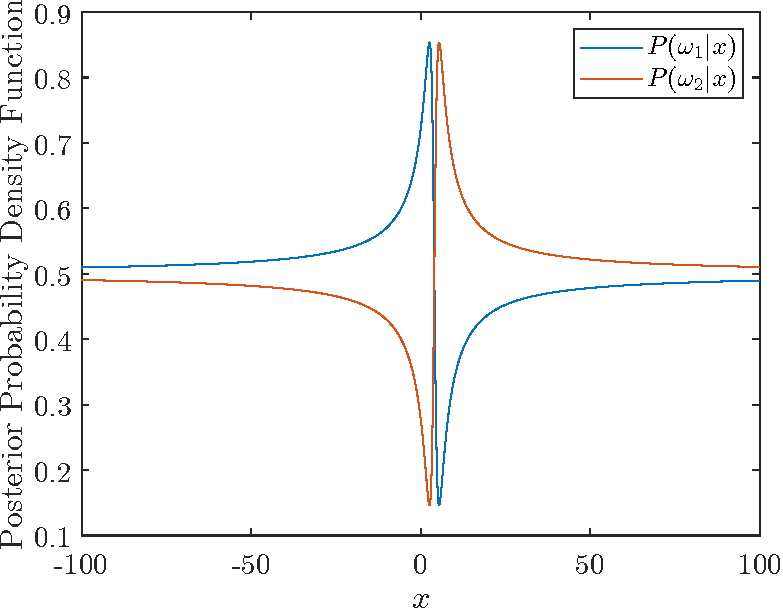
\includegraphics[width=10cm]{postpdf.pdf}
  \caption{后验概率}
  \label{fig:postpdf}
\end{figure}

1.4. Assuming $P(\omega_1) = P(\omega_2)$, how do $P(\omega_1|x)$ and $P(\omega_2|x)$ behave as $x \rightarrow -\infty$? $x\rightarrow +\infty$? Explain.

解: 由图 \ref{fig:postpdf} 可知, 当 $x \rightarrow \pm\infty$ 时, $P(\omega_1|x)=P(\omega_2|x)=\dfrac{1}{2}$, 证明如下.

对式 (\ref{eq:postpdf}) 取极限可得
\begin{equation}
  \lim_{x\to\pm\infty}P(\omega_1|x)
  =\lim_{x\to\pm\infty}\frac{1+\left(\dfrac{x-a_2}{b}\right)^2}{1+\left(\dfrac{x-a_1}{b}\right)^2+1+\left(\dfrac{x-a_2}{b}\right)^2}=\frac{1}{2}
\end{equation}

则有
\begin{equation}
  \lim_{x\to\pm\infty}P(\omega_2|x)
  =\frac{1}{2}
\end{equation}

2. Consider Neyman-Pearson criteria for two Cauchy distributions in one dimension described in Problem 1. Assume a zero-one error loss, and for simplicity $a_{2}>a_{1}$, the same ``width" $b$, and equal priors.

2.1. Suppose the maximum acceptable error rate for classifying a pattern that is actually in $\omega_{1}$ as if it were in $\omega_{2}$ is $E_{1}$. Determine the decision boundary in terms of the variables given.

解: 本题要求考虑 Neyman-Pearson 准则, 则边界并不一定是单边边界, 以下为大部分错误解法. 

设边界点为 $t$, 由 $a_{2}>a_{1}$ 可知
\begin{equation}
  R_1=(-\infty,t),\quad R_2=(t,\infty)
\end{equation}

又先验概率相等, 则
\begin{equation}
  P(\omega_1)=p(\omega_2)=\frac{1}{2}
\end{equation}

故第一类错误率
\begin{equation}
  \begin{aligned}
    E_1
    &=\int_t^\infty p(x|\omega_1)P(\omega_1)\mathrm{d}x\\
    &=\frac{1}{2}\int_t^\infty \frac{1}{\pi b} \cdot \frac{1}{1+\left(\dfrac{x-a_1}{b}\right)^2}\mathrm{d}x\\
    &=\frac{1}{2\pi}\int_{(t-a_1)/b}^\infty \frac{1}{1+u^2}\mathrm{d}u,\quad u=\dfrac{x-a_1}{b}\\
    &=\frac{1}{2\pi}\arctan(u)\Big|_{(t-a_1)/b}^\infty\\
    &=\frac{1}{2\pi}\left[\frac{\pi}{2}-\arctan\left(\frac{t-a_1}{b}\right)\right]
  \end{aligned}
\end{equation}

即
\begin{equation}
  \arctan\left(\frac{t-a_1}{b}\right)=\frac{\pi}{2}-2\pi E_1
\end{equation}

两边取正切可得
\begin{equation}
  \frac{t-a_1}{b}=\tan\left(\frac{\pi}{2}-2\pi E_1\right)=\cot(2\pi E_1)
\end{equation}

故
\begin{equation}
  t=a_1+b\cot(2\pi E_1)=a_1+\frac{b}{\tan(2\pi E_1)}
\end{equation}

正确解法应为, 考虑两类错误
\begin{equation}
  \begin{aligned}
    P_1(e)&=\int_{\Rc_2}p(x|\omega_1)\mathrm{d}x=E_1\\
    P_2(e)&=\int_{\Rc_1}p(x|\omega_2)\mathrm{d}x\\
  \end{aligned}
\end{equation}

最小化 $P_2(e)$ 等价于
\begin{equation}
  \min\gamma=P_2(e)+\lambda(P_1(e)-E_1)
\end{equation}

对 $\lambda$ 和 $\Rc_2$ 边界求导等于 0, 有
\begin{equation}
    \lambda=\frac{p(x|\omega_2)}{p(x|\omega_1)}=\frac{b^2+(x-a_1)^2}{b^2+(x-a_2)^2}
\end{equation}
\begin{equation}
  \int_{\Rc_2}p(x|\omega_1)\mathrm{d}x=E_1
\end{equation}

则决策边界为
\begin{equation}
  t_{1,2}=\frac{(a_1-\lambda a_2)\pm\sqrt{\lambda(a_1-a_2)^2-b^2(\lambda-1)^2}}{1-\lambda}
\end{equation}

2.2. For this boundary, what is the error rate for classifying $\omega_{2}$ as $\omega_{1}$?

解: 第二类错误率为
\begin{equation}
  \begin{aligned}
    E_2
    &=\int_{-\infty}^{\top} p(x|\omega_2)P(\omega_2)\mathrm{d}x\\
    &=\frac{1}{2}\int_{-\infty}^{\top}\frac{1}{\pi b} \cdot \frac{1}{1+\left(\dfrac{x-a_2}{b}\right)^2}\mathrm{d}x\\
    &=\frac{1}{2\pi}\int_{-\infty}^{(t-a_2)/b}\frac{1}{1+u^2}\mathrm{d}u\\
    &=\frac{1}{2\pi}\left[\arctan\left(\frac{t-a_2}{b}\right)+\frac{\pi}{2}\right]
  \end{aligned}
\end{equation}

2.3. What is the overall error rate under zero-one loss?

解: 总错误率为
\begin{equation}
  E=E_1+E_2=E_1+\frac{1}{2\pi}\left[\arctan\left(\frac{t-a_2}{b}\right)+\frac{\pi}{2}\right]
\end{equation}

2.4. Apply your results to the specific case $b=1$ and $a_{1}=-1, a_{2}=1$ and $E_{1}=0.1$.

解: 代入数值得边界点为
\begin{equation}
  t=a_1+\frac{b}{\tan(2\pi E_1)}=-1+\frac{1}{\tan(2\pi\times0.1)}\approx0.376
\end{equation}

则总错误率为
\begin{equation}
  \begin{aligned}
    E
    &=E_1+\frac{1}{2\pi}\left[\arctan\left(\frac{t-a_2}{b}\right)+\frac{\pi}{2}\right]\\
    &=0.1+\frac{1}{2\pi}\left[\arctan\left(\frac{0.376-1}{1}\right)+\frac{\pi}{2}\right]\\
    &\approx0.261\\
  \end{aligned}
\end{equation}

2.5. Compare your result to the Bayes error rate (i.e. without the Neyman-Pearson conditions).

解: 对于 Bayes 决策, 分界点为
\begin{equation}
  t=\frac{a_1+a_2}{2}=\frac{-1+1}{2}=0
\end{equation}

故 Bayes 错误率为
\begin{equation}
  \begin{aligned}
    E_B
    &=\int_{-\infty}^{\top} p(x|\omega_2)P(\omega_2)\mathrm{d}x+\int_t^\infty p(x|\omega_1)P(\omega_1)\mathrm{d}x\\
    &=\frac{1}{2\pi}\left[\frac{\pi}{2}-\arctan\left(\frac{t-a_1}{b}\right)\right]+\frac{1}{2\pi}\left[\arctan\left(\frac{t-a_2}{b}\right)+\frac{\pi}{2}\right]\\
    &=\frac{1}{2}-\frac{1}{2\pi}\arctan\left(\frac{0+1}{1}\right)+\frac{1}{2\pi}\arctan\left(\frac{0-1}{1}\right)\\
    &=\frac{1}{4}\\
  \end{aligned}
\end{equation}

由 $E_B<E$ 可知 Bayes 决策错误率小于 Neyman-Pearson 决策错误率.

3. In many pattern classification problems one has the option either to assign the pattern to one of $c$ classes, or to \emph{reject} it as being unrecognizable. If the cost for rejects is not too high, rejection may be a desirable action. Let
\begin{equation}
  \lambda(\alpha_i|\omega_j)=
  \left\{
    \begin{array}{ll}
    0         & i=j, \quad i,j=1,2,\cdots, c  \\
    \lambda_r & i = c+1 \\
    \lambda_s & \mathrm{otherwise},  
    \end{array}
  \right.
\end{equation}

where $\lambda_r$ is the loss incurred for choosing the $(c+1)$th action, rejection, and $\lambda_s$ is the loss incurred for making a substitution error. Show that the minimum risk is obtained if we decide $\omega_i$ if $P(\omega_i|\bm{x})\gs P(\omega_j|\bm{x})$ for all $j$ and if $P(\omega_i|\bm{x})\gs 1-\lambda_r/\lambda_s$, and reject otherwise. What happens if $\lambda_r=0$? What happens if $\lambda_r>\lambda_s$?

解: 令
\begin{equation}
  m=\argmax_{j=1,2,\cdots,c}P(\omega_j|x)
\end{equation}

即 $\omega_m$ 表示后验概率最大的类别, 分类讨论. 

当选择 $\omega_m$ 时, 风险为
\begin{equation}
  R_m=\lambda_s\sum_{j\neq m}P(\omega_j|x)=\lambda_s[1-P(\omega_m|x)]
\end{equation}

当选择其他类别 $\omega_k$, $k\neq m$ 时, 风险为
\begin{equation}
  R_k=\lambda_s\sum_{j\neq k}P(\omega_j|x)=\lambda_s[1-P(\omega_k|x)]\gs\lambda_s[1-P(\omega_m|x)]
\end{equation}

当选择拒绝时, 风险为
\begin{equation}
  R_r=\lambda_r
\end{equation}

所以最小风险为
\begin{equation}
  \begin{aligned}
    R
    &=\min\{R_m,R_k,R_r\}\\
    &=\min\{\lambda_s[1-P(\omega_m|x)],\lambda_r\}\\
  \end{aligned}
\end{equation}

当 $\lambda_s[1-P(\omega_m|x)]\ls\lambda_r$, 即
\begin{equation}
  P(\omega_m|x)\gs1-\frac{\lambda_r}{\lambda_s}
\end{equation}

时, 选择 $\omega_m$ 风险最小, 否则选择拒绝风险最小.

若 $\lambda_r=0$, 则选择拒绝风险最小, 会拒绝所有样本.

若 $\lambda_r>\lambda_s$, 则选择最大后验概率类别 $\omega_m$ 风险最小, 不会拒绝任何样本.

4. Consider a two-category classification problem in two dimensions. Given the following conditions, calculate the Bayes decision boundary respectively and plot them in the coordinate space (with computer or by hand). You should indicate the mean point of each category.

4.1. We set $p(\bm{x}|\omega_1)\sim N(\bm{0},\bm{I})$, $p(\bm{x}|\omega_2)\sim N\left((1,1)^{\top},\bm{I}\right)$ and $P(\omega_1)=P(\omega_2)=0.5$. 

解: 忽略类别无关项, 判别函数为
\begin{equation}
  g_i(\vx)=-\frac{1}{2\sigma^2}(\vx-\vmu_i)^{\top}(\vx-\vmu_i)
\end{equation}

决策面满足
\begin{equation}
  g_i(\vx)=g_j(\vx)
\end{equation}

故
\begin{equation}
  -\frac{1}{2\sigma^2}(\vx-\vmu_i)^{\top}(\vx-\vmu_i)=-\frac{1}{2\sigma^2}(\vx-\vmu_j)^{\top}(\vx-\vmu_j)
\end{equation}

化简得
\begin{equation}
  -2\vx^{\top}\vmu_i+\vmu_i^{\top}\vmu_i=-2\vx^{\top}\vmu_j+\vmu_j^{\top}\vmu_j
\end{equation}

即
\begin{equation}
  (\vmu_i-\vmu_j)^{\top}\vx-\frac{1}{2}(\vmu_i^{\top}\vmu_i-\vmu_j^{\top}\vmu_j)=0
\end{equation}

代入数据得
\begin{equation}
  x_1+x_2-1=0
\end{equation}

决策面如图 \ref{fig:mvnpdf-1} 所示.

\begin{figure}
  \centering
  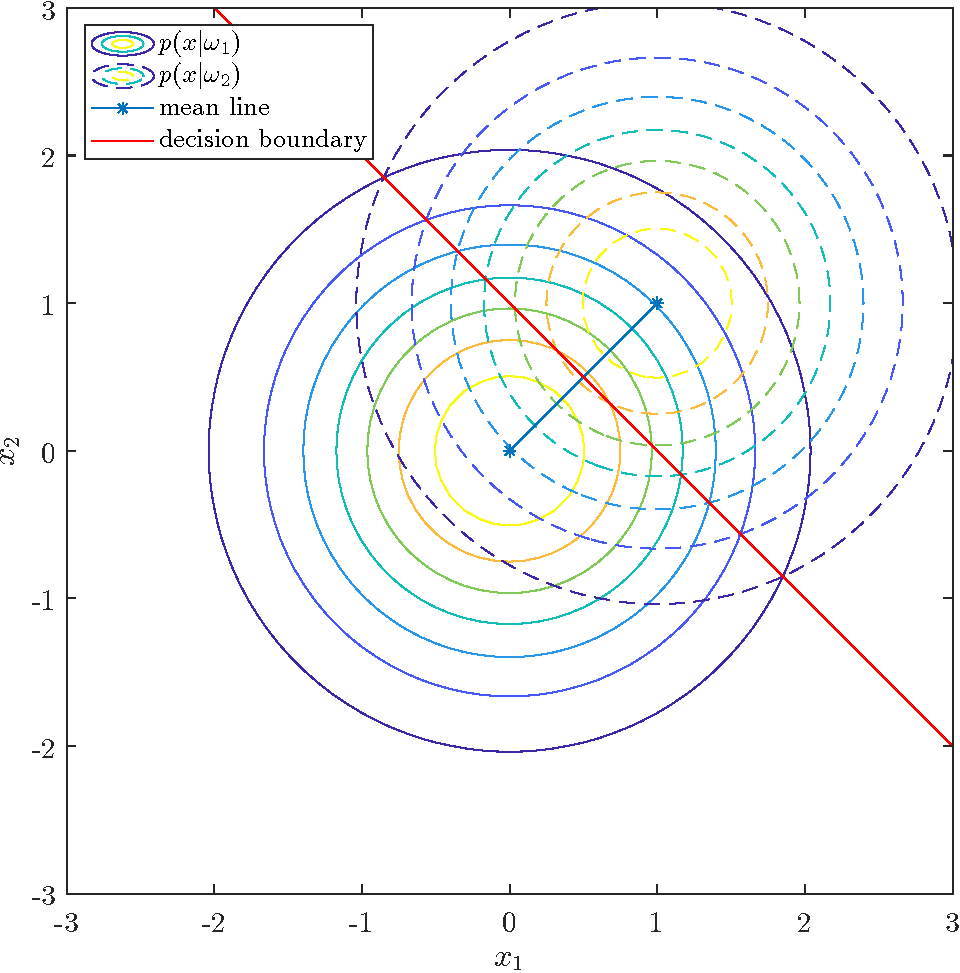
\includegraphics[width=10cm]{mvnpdf-1.pdf}
  \caption{决策面}
  \label{fig:mvnpdf-1}
\end{figure}

4.2. We set $p(\bm{x}|\omega_1)\sim N(\bm{0},\bm{I})$, $p(\bm{x}|\omega_2)\sim N\left((1,1)^{\top},\bm{I}\right)$ and $P(\omega_1)=0.2, P(\omega_2)=0.8$.

解: 忽略类别无关项, 判别函数为
\begin{equation}
  g_i(\vx)=-\frac{1}{2\sigma^2}(\vx-\vmu_i)^{\top}(\vx-\vmu_i)+\ln P(\omega_i)
\end{equation}

决策面满足
\begin{equation}
  g_i(\vx)=g_j(\vx)
\end{equation}

故
\begin{equation}
  -\frac{1}{2\sigma^2}(\vx-\vmu_i)^{\top}(\vx-\vmu_i)+\ln P(\omega_i)=-\frac{1}{2\sigma^2}(\vx-\vmu_j)^{\top}(\vx-\vmu_j)+\ln P(\omega_j)
\end{equation}

化简得
\begin{equation}
  -2\vx^{\top}\vmu_i+\vmu_i^{\top}\vmu_i-2\sigma^2\ln P(\omega_i)
  =-2\vx^{\top}\vmu_j+\vmu_j^{\top}\vmu_j-2\sigma^2\ln P(\omega_j)
\end{equation}

即
\begin{equation}
  (\vmu_i-\vmu_j)^{\top}\vx-\frac{1}{2}(\vmu_i^{\top}\vmu_i-\vmu_j^{\top}\vmu_j)+\sigma^2\ln\frac{P(\omega_i)}{P(\omega_j)}=0
\end{equation}

代入数据得
\begin{equation}
  x_1+x_2-1+\ln4=0
\end{equation}

决策面如图 \ref{fig:mvnpdf-2} 所示.

\begin{figure}
  \centering
  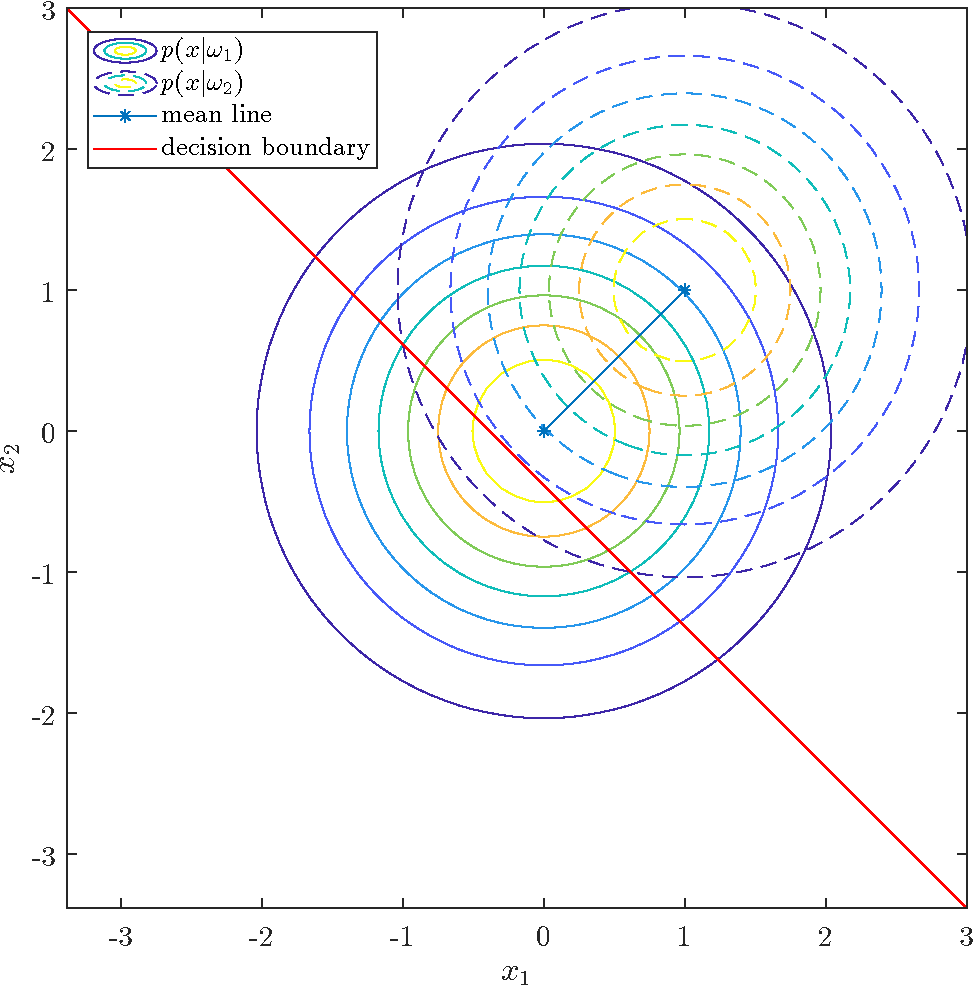
\includegraphics[width=10cm]{mvnpdf-2.pdf}
  \caption{决策面}
  \label{fig:mvnpdf-2}
\end{figure}

4.3. We set $p(\bm{x}|\omega_1)\sim N\left(\bm{0},\begin{bmatrix} 1 & 1 \\ 1 & 2 \end{bmatrix}\right)$, $p(\bm{x}|\omega_2)\sim N\left((1,1)^{\top},\begin{bmatrix} 1 & 1 \\ 1 & 2 \end{bmatrix}\right)$ and $P(\omega_1)=P(\omega_2)=0.5$.

解: 忽略类别无关项, 判别函数为
\begin{equation}
  g_i(\vx)=-\frac{1}{2}(\vx-\vmu_i)^{\top}\mSigma^{-1}(\vx-\vmu_i)
\end{equation}

决策面满足
\begin{equation}
  g_i(\vx)=g_j(\vx)
\end{equation}

故
\begin{equation}
  -\frac{1}{2}(\vx-\vmu_i)^{\top}\mSigma^{-1}(\vx-\vmu_i)=-\frac{1}{2}(\vx-\vmu_j)^{\top}\mSigma^{-1}(\vx-\vmu_j)
\end{equation}

化简得
\begin{equation}
  -2\vx^{\top}\mSigma^{-1}\vmu_i+\vmu_i^{\top}\mSigma^{-1}\vmu_i
  =-2\vx^{\top}\mSigma^{-1}\vmu_j+\vmu_j^{\top}\mSigma^{-1}\vmu_j
\end{equation}

即
\begin{equation}
  (\vmu_i-\vmu_j)^{\top}\mSigma^{-1}\vx-\frac{1}{2}(\vmu_i^{\top}\mSigma^{-1}\vmu_i-\vmu_j^{\top}\mSigma^{-1}\vmu_j)=0
\end{equation}

代入数据得
\begin{equation}
  x_1-\frac{1}{2}=0
\end{equation}

决策面如图 \ref{fig:mvnpdf-3} 所示.

\begin{figure}
  \centering
  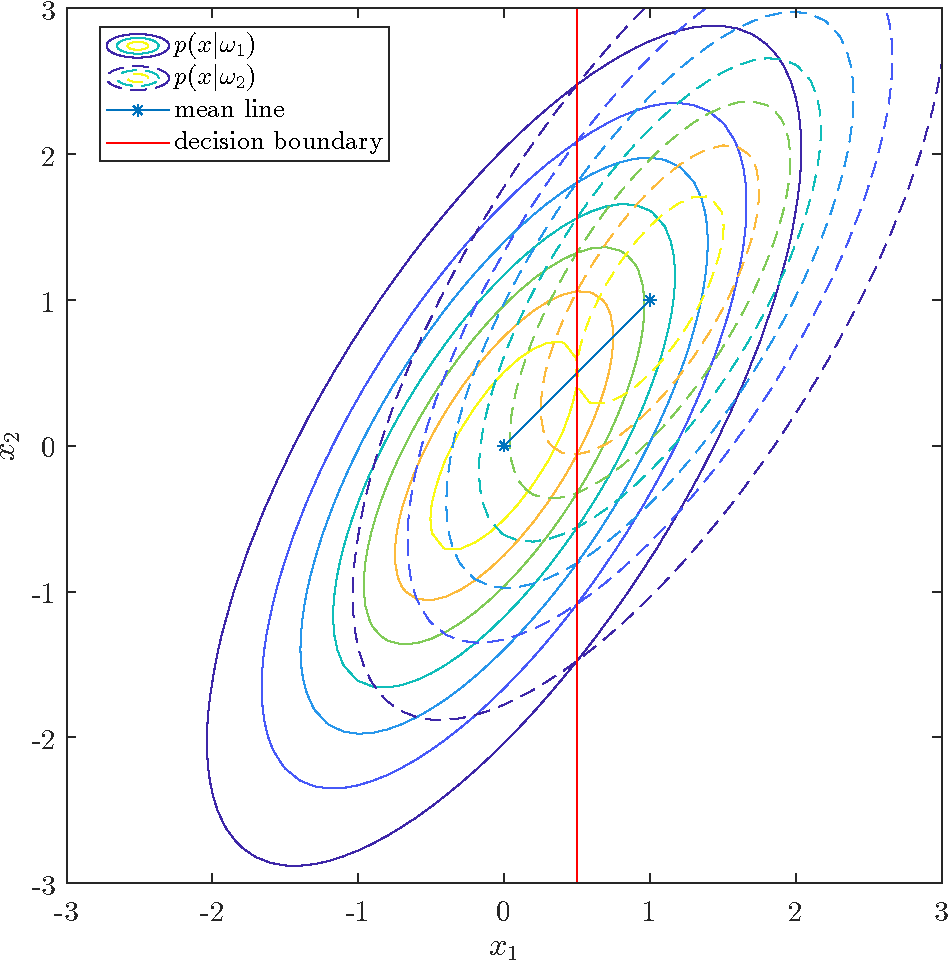
\includegraphics[width=10cm]{mvnpdf-3.pdf}
  \caption{决策面}
  \label{fig:mvnpdf-3}
\end{figure}

4.4. We set $p(\bm{x}|\omega_1)\sim N\left(\bm{0},\begin{bmatrix} 1 & 0 \\ 0 & 2 \end{bmatrix}\right)$, $p(\bm{x}|\omega_2)\sim N\left((1,1)^{\top},\begin{bmatrix} 2 & 0 \\ 0 & 1 \end{bmatrix}\right)$ and $P(\omega_1)=P(\omega_2)=0.5$.

解: 忽略类别无关项, 判别函数为
\begin{equation}
  g_i(\vx)=-\frac{1}{2}(\vx-\vmu_i)^{\top}\mSigma_i^{-1}(\vx-\vmu_i)-\frac{1}{2}\ln|\mSigma_i|
\end{equation}

决策面满足
\begin{equation}
  g_i(\vx)=g_j(\vx)
\end{equation}

故
\begin{equation}
  -\frac{1}{2}(\vx-\vmu_i)^{\top}\mSigma_i^{-1}(\vx-\vmu_i)-\frac{1}{2}\ln|\mSigma_i|=-\frac{1}{2}(\vx-\vmu_j)^{\top}\mSigma_j^{-1}(\vx-\vmu_j)-\frac{1}{2}\ln|\mSigma_j|
\end{equation}

化简得
\begin{equation}
  \vx^{\top}\mSigma_i^{-1}\vx-2\vx^{\top}\mSigma_i^{-1}\vmu_i+\vmu_i^{\top}\mSigma_i^{-1}\vmu_i+\ln|\mSigma_i|
  =\vx^{\top}\mSigma_j^{-1}\vx-2\vx^{\top}\mSigma_j^{-1}\vmu_j+\vmu_j^{\top}\mSigma_j^{-1}\vmu_j+\ln|\mSigma_j|
\end{equation}

即
\begin{equation}
  \vx^{\top}(\mSigma_j^{-1}-\mSigma_i^{-1})\vx+2(\vmu_i\mSigma_i^{-1}-\vmu_j\mSigma_j^{-1})^{\top}\vx-(\vmu_i^{\top}\mSigma_i^{-1}\vmu_i-\vmu_j^{\top}\mSigma_j^{-1}\vmu_j)-(\ln|\mSigma_i|-\ln|\mSigma_j|)=0
\end{equation}

代入数据得
\begin{equation}
  \frac{1}{2}x_1^2-\frac{1}{2}x_2^2+x_1+2x_2-\frac{3}{2}=0
\end{equation}

化简得
\begin{equation}
  x_1^2-x_2^2+2x_1+4x_2-3=0
\end{equation}

即
\begin{equation}
  (x_1+1)^2-(x_2-2)^2=0
\end{equation}

即
\begin{equation}
  |x_1+1|=|x_2-2|
\end{equation}

决策面如图 \ref{fig:mvnpdf-4} 所示.

\begin{figure}[t]
  \centering
  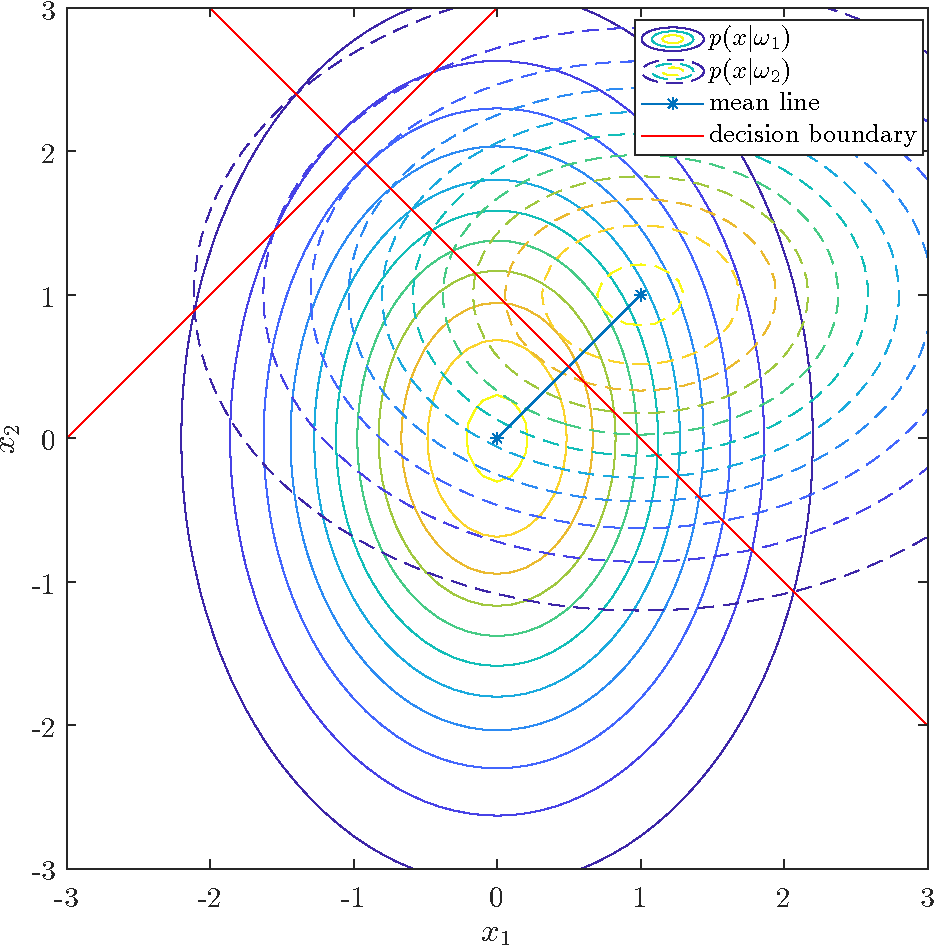
\includegraphics[width=10cm]{mvnpdf-4.pdf}
  \caption{决策面}
  \label{fig:mvnpdf-4}
\end{figure}

\section*{Naive Bayes}


5. Consider a simple learning problem of determining whether Alice and Bob from CA will go to hiking or not, $Y:Hike\in\{T,F\}$ given the weather conditions $X_1:Sunny\in\{T,F\}$ and $X_2:Windy\in\{T,F\}$ by a Naive Bayes classifier. Using training data, we estimated the parameters $P(Hike) = 0.5$, $P(Sunny|Hike) = 0.9$, $P(Windy|\neg Hike) = 0.8$, $P(Windy|Hike) = 0.3$ and $P(Sunny|\neg Hike) = 0.4$. Assume that the true distributions of $X_1$, $X_2$, and $Y$ satisfy the Naive Bayes assumption of conditional independence with the above parameters.

5.1. Assume Sunny and Windy are truly independent given Hike. Write down the Naive Bayes decision rule for this problem using both attributes Sunny and Windy.

解: 已知 $P(Hike) = 0.5$, 则 $P(\neg Hike)=P(Hike)=0.5$. 

由 Bayes 公式结合条件独立的假设可得
\begin{equation}
  \begin{aligned}
    P(Hike|Sunny,Windy)&=\frac{0.9\times0.3}{0.9\times0.3+0.4\times0.8}=0.4576\\
    P(Hike|Sunny,\neg Windy)&=\frac{0.9\times0.7}{0.9\times0.7+0.4\times0.2}=0.8873\\
    P(Hike|\neg Sunny,Windy)&=\frac{0.1\times0.3}{0.1\times0.3+0.6\times0.8}=0.0588\\
    P(Hike|\neg Sunny,\neg Windy)&=\frac{0.1\times0.7}{0.1\times0.7+0.6\times0.2}=0.3684\\
  \end{aligned}
\end{equation}

所以
\begin{equation}
  \begin{aligned}
    P(Hike|Sunny,Windy)&<P(\neg Hike|Sunny,Windy)\\
    P(Hike|Sunny,\neg Windy)&>P(\neg Hike|Sunny,\neg Windy)\\
    P(Hike|\neg Sunny,Windy)&<P(\neg Hike|\neg Sunny,Windy)\\
    P(Hike|\neg Sunny,\neg Windy)&<P(\neg Hike|\neg Sunny,\neg Windy)\\
  \end{aligned}
\end{equation}

因此 Bayes 决策规则为
\begin{equation}
  \begin{aligned}
    (Sunny,Windy)&\to\neg Hike\\
    (Sunny,\neg Windy)&\to Hike\\
    (\neg Sunny,Windy)&\to\neg Hike\\
    (\neg Sunny,\neg Windy)&\to\neg Hike\\
  \end{aligned}
\end{equation}

5.2. Given the decision rule above, what is the expected error rate of the Naive Bayes classifier? (The expected error rate is the probability that each class generates an observation where the decision rule is incorrect.)

解: 由 Bayes 决策规则可知, 错误率为
\begin{equation}
  \begin{aligned}
    E
    &=P(Hike)[1-P(Sunny,\neg Windy|Hike)]+P(\neg Hike)P(Sunny,\neg Windy|\neg Hike)\\
    &=0.5\times(1-0.9\times0.7)+0.5\times0.4\times0.2\\
    &=0.225\\
  \end{aligned}
\end{equation}

5.3. What is the joint probability that Alice and Bob go to hiking and the weather is sunny and windy, that is $P(Sunny,Windy,Hike)$?

解: 由条件乘法公式与条件独立性可知, 联合概率密度为
\begin{equation}
  \begin{aligned}
    P(Sunny,Windy,Hike)
    &=P(Hike)P(Sunny,Windy|Hike)\\
    &=P(Hike)P(Sunny|Hike)P(Windy|Hike)\\
    &=0.5 \times 0.9 \times 0.3\\
    &=0.135\\
  \end{aligned}
\end{equation}

5.4. Next, suppose that we gather more information about weather conditions and introduce a new feature denoting whether the weather is $X_3$: Rainy or not. Assume that each day the weather in CA can be either Rainy or Sunny. That is, it can not be both Sunny and Rainy (similarly, it can not be $\neg Sunny$ and $\neg Rainy$). In the above new case, are any of the Naive Bayes assumptions violated? Why (not)? What is the joint probability that Alice and Bob go to hiking and the weather is sunny, windy and not rainy, that is $P(Sunny,Windy,\neg Rainy,Hike)$?

解: 确有 Naive Bayes 的假设不成立, 事实上
\begin{equation}
  P(Sunny,Windy,Rainy|Hike)=0
\end{equation}

而
\begin{equation}
  \begin{aligned}
     &~P(Sunny|Hike)P(Windy|Hike)P(Rainy|Hike)\\
    =&~P(Sunny|Hike)P(Windy|Hike)P(\neg Sunny|Hike)\\
    =&~0.9\times0.3\times0.1\\
    =&~0.027\\
  \end{aligned}
\end{equation}

所以
\begin{equation}
  P(Sunny,Windy,Rainy|Hike)\neq P(Sunny|Hike)P(Windy|Hike)P(Rainy|Hike)
\end{equation}

故 Naive Bayes 的条件独立性假设不成立.

由题干假设以及条件乘法公式可知, 联合概率密度为
\begin{equation}
  \begin{aligned}
    P(Sunny,Windy,\neg Rainy,Hike)
    &=P(Sunny,Windy,Hike)\\
    &=P(Hike)P(Sunny,Windy|Hike)\\
    &=P(Hike)P(Sunny|Hike)P(Windy|Hike)\\
    &=0.5 \times 0.9 \times 0.3\\
    &=0.135\\
  \end{aligned}
\end{equation}


5.5. What is the expected error rate when the Naive Bayes classier uses all three attributes? Will the performance of Naive Bayes be improved by observing the new attribute Rainy? Explain why. 

解: 考虑三种因素的 Bayes 决策规则为
\begin{equation}
  \begin{aligned}
    (Sunny,Windy,\neg Rainy)&\to\neg Hike\\
    (Sunny,\neg Windy,\neg Rainy)&\to Hike\\
    (\neg Sunny,Windy,Rainy)&\to\neg Hike\\
    (\neg Sunny,\neg Windy,Rainy)&\to\neg Hike\\
  \end{aligned}
\end{equation}

错误率为
\begin{equation}
  \begin{aligned}
    \tilde{E}
    &=P(Hike)[1-P(Sunny,\neg Windy,\neg Rainy|Hike)]+P(\neg Hike)P(Sunny,\neg Windy,\neg Rainy|\neg Hike)\\
    &=P(Hike)[1-P(Sunny,\neg Windy|Hike)]+P(\neg Hike)P(Sunny,\neg Windy|\neg Hike)\\
    &=0.5\times(1-0.9\times0.7)+0.5\times0.4\times0.2\\
    &=0.225\\
  \end{aligned}
\end{equation}

由 $\tilde{E}=E$ 可知, 增加新要素 Rainy 并不能改进 Naive Bayes 的性能, 因为 Rainy 信息可以直接从 Sunny 信息获得, 本质上并未真正增加新的信息.

\section*{ROC Analysis}

6. The purpose of this assignment is to learn the theory and practical applications of ROC analysis. Therefore you should first read a paper about ROC curves~\cite{b1} that is available in this homework zip (especially pay attention to section 1-5 and 7-8). In the following task you will work on a given theoretical example of two classifier ($C_1$ and $C_2$). We have a set of samples that we wish to classify in one of two classes and a ground truth class of each sample (denoted as 0 and 1). For each sample a classifier gives a score based on which we can determine to which class should be the sample belong to (score closer to 0 means class 0, score closer to 1 means class 1). Below are the results for 8 samples, their ground truth values ($S_{\text{id}}$) and the score values for both classifiers ($S_{C_1}$ and $S_{C_2}$).

\begin{equation}
  \begin{aligned}
    S_{\text{id}} &= [1\quad 0 \quad 1 \quad 1 \quad 1 \quad 0 \quad 0 \quad 0]\\
    S_{C_1} &= [0.5\quad 0.3 \quad 0.6 \quad 0.22 \quad 0.4 \quad 0.51 \quad 0.2 \quad 0.33] \\
    S_{C_2} &= [0.04\quad 0.1 \quad 0.68 \quad 0.22 \quad 0.4 \quad 0.11 \quad 0.8 \quad 0.53]\\
  \end{aligned}
\end{equation}

For the example above calculate (by hand) and draw the ROC curves for classifier $C_1$ as well as classifier $C_2$. Also calculate the area under the curve (AUC) for both classifier. For the classifier $C_1$ select a decision threshold (working points) $\theta_{1}=0.33$. For the classifier $C_2$ select a decision threshold  $\theta_{2}=0.1$.  Based on theory from~\cite{b1} decide which classifier is better in the selected working points and motivate your decision. Which working point is optimal for each classifier? 

解: 分别对两个分类器的分数进行排序, 计算相应的真阳性率和假阳性率, 分类器1的计算结果如表 \ref{tab:classifier1} 所示, 分类器2的计算结果如表 \ref{tab:classifier2} 所示.

\begin{table}
  \centering
  \begin{minipage}{0.4\textwidth}
    \centering
    \caption{分类器1}
    \label{tab:classifier1}
    \begin{tabular}{cccc}
      \toprule
      Class & Score & FP Rate & TP Rate \\
      \midrule
      1     & 0.6   & 0       & 1/4     \\
      0     & 0.51  & 1/4     & 1/4     \\
      1     & 0.5   & 1/4     & 2/4     \\
      1     & 0.4   & 1/4     & 3/4     \\
      0     & 0.33  & 2/4     & 3/4     \\
      0     & 0.3   & 3/4     & 3/4     \\
      1     & 0.22  & 3/4     & 1       \\
      0     & 0.2   & 1       & 1       \\
      \bottomrule   
    \end{tabular}
  \end{minipage}
  \begin{minipage}{0.4\textwidth}
    \centering
    \caption{分类器2}
    \label{tab:classifier2}
    \begin{tabular}{cccc}
      \toprule
      Class & Score & FP Rate & TP Rate \\
      \midrule
      0     & 0.8   & 1/4     & 0       \\
      1     & 0.68  & 1/4     & 1/4     \\
      0     & 0.53  & 2/4     & 1/4     \\
      1     & 0.4   & 2/4     & 2/4     \\
      1     & 0.22  & 2/4     & 3/4     \\
      0     & 0.11  & 3/4     & 3/4     \\
      0     & 0.1   & 1       & 3/4     \\
      1     & 0.04  & 1       & 1       \\
      \bottomrule   
    \end{tabular}
  \end{minipage}
\end{table}

根据计算结果, 绘制两个分类器的 ROC 曲线分别如图 \ref{fig:roc1} 和图 \ref{fig:roc2} 所示.

\begin{figure}[htbp]
  \centering
  \begin{minipage}[t]{0.48\textwidth}
  \centering
  \begin{tikzpicture}
    \coordinate (P0) at (0,0);
    \draw[-latex] (0,0) -- (5,0);
    \draw (2.5,-0.5) node[below] {FP Rate};
    \draw[-latex] (0,0) -- (0,5);
    \draw (-0.5,2.5) node[rotate=90,above] {TP Rate};
    \draw (P0) node [below left]{0};
    \draw[line width=1pt] plot[mark=*] coordinates {(0,0) (0,1) (1,1) (1,2) (1,3) (2,3) (3,3) (3,4) (4,4)};
    \draw[dashed] (4,4) -- (0,4) node[left] {1};
    \draw[dashed] (4,4) -- (4,0) node[below] {1};
  \end{tikzpicture}
  \caption{分类器1 ROC 曲线}
  \label{fig:roc1}
  \end{minipage}
  \begin{minipage}[t]{0.48\textwidth}
  \centering
  \begin{tikzpicture}
    \coordinate (P0) at (0,0);
    \draw[-latex] (0,0) -- (5,0);
    \draw (2.5,-0.5) node[below] {FP Rate};
    \draw[-latex] (0,0) -- (0,5);
    \draw (-0.5,2.5) node[rotate=90,above] {TP Rate};
    \draw (P0) node [below left]{0};
    \draw[line width=1pt] plot[mark=*] coordinates {(0,0) (1,0) (1,1) (2,1) (2,2) (2,3) (3,3) (4,3) (4,4)};
    \draw[dashed] (4,4) -- (0,4) node[left] {1};
    \draw[dashed] (4,4) -- (4,0) node[below] {1};
  \end{tikzpicture}
  \caption{分类器2 ROC 曲线}
  \label{fig:roc2}
  \end{minipage}
\end{figure}

由图 \ref{fig:roc1} 和图 \ref{fig:roc2} 可得两个分类器的 AUC 分别为
\begin{equation}
  \begin{aligned}
    \mathrm{AUC}_1&=1-5\times\frac{1}{4}\times\frac{1}{4}=\frac{11}{16}\\
    \mathrm{AUC}_2&=7\times\frac{1}{4}\times\frac{1}{4}=\frac{7}{16}\\
  \end{aligned}
\end{equation}

由 $\theta_{1}=0.33$ 和 $\theta_{2}=0.1$ 可知分类器1和分类器2的工作点分别为 (2/4, 3/4) 和 (1, 3/4), 两个工作点的真阳性率相等, 但是分类器1的假阳性率更小, 故在选定工作点处分类器1更好.

越靠近 ROC 曲线左上角的工作点越好, 故对分类器1来说, 工作点 (1/4, 3/4) 最好, 相应的阈值为 $\theta_{1}=0.4$; 对分类器2来说, 工作点 (2/4, 3/4) 最好, 相应的阈值为 $\theta_{2}=0.22$.

% Reference
\begin{thebibliography}{1}
  \bibitem{b1}{T. Fawcett. An introduction to ROC analysis. Pattern Recognition Letters, 27(8):861-874, 2006.}
\end{thebibliography}

\end{document}
